\documentclass[a4paper,11pt]{article}
\usepackage[margin=1in]{geometry}
\usepackage{hyperref, setspace, lineno, amsmath, amssymb, longtable}
\usepackage{float} %% fix graphs at where they should be
\usepackage{amsmath}
\usepackage{amssymb}
\usepackage{textcomp}
\usepackage{amsthm}
\usepackage{graphicx}
\usepackage{enumerate}
\usepackage{booktabs}
\usepackage{threeparttable}
\usepackage[round]{natbib} 
\bibliographystyle{plainnat}

%you can add more packages using the same code above

%------------------

%\setlength{\topmargin}{0.0in}
%\setlength{\textheight}{10in}
%\setlength{\oddsidemargin}{0.0in}
%\setlength{\evensidemargin}{0.0in}
%\setlength{\textwidth}{6.5in}

%-------------------
\newtheorem{theorem}{Theorem}[section]
\newtheorem{proposition}[theorem]{Proposition}
\newtheorem{lemma}[theorem]{Lemma}
\newtheorem{corollary}[theorem]{Corollary}
\newtheorem{conjecture}[theorem]{Conjecture}


\theoremstyle{definition}
\newtheorem{definition}[theorem]{Definition}
\newtheorem*{example}{Example}

%------------------
\newcommand{\ReportAuthor}{Yuqing Zhou}
\newcommand{\ReportAffil}{Department of Life Sciences, Faculty of Natural Sciences,\\Imperial College London}
\newcommand{\ReportTitle}{Comparison of Models for Fitting Population Growth Curves}


%------------------
%Everything before begin document is called the pre-amble and sets out how the document will look
%It is recommended you don't touch the pre-amble until you are familiar with LateX
\setlength{\marginparwidth}{2cm}
\doublespacing



\begin{document}
    %\maketitle
    \begin{titlepage}
        \vspace{10pt}
        \begin{figure}[!ht]
            \centering
                \begin{center}
                     
\includegraphics[width=\linewidth]{../data/IMP_LOGO.jpg}
                \end{center}
        \end{figure}

        \vspace{5pt}
    	\begin{center}
            \Huge\textbf{\ReportTitle}\\
        \end{center}
        
        \begin{center}
        \vspace{\fill}
            \LARGE\ReportAuthor\\
		    \vspace{6pt}
            \Large\ReportAffil
        \end{center}
        	
        \begin{center}
        \vspace{\fill}
    	    \normalsize{March, 2020}
        \end{center}       
        \begin{flushright}
		    \normalsize Approximate Word Count: 2000%% insert approx word count
	    \end{flushright}
    \end{titlepage}
    

\title{Comparison of Models for fitting Population Growth Curves}
\author{Yuqing Zhou\ (CID: 01807289)}

\date{}
\maketitle

\begin{abstract}
Predictive modelling of microbial growth pattern has become increasingly important in the field of food microbiology. Several mechanistic and phenomenological models(logistic, Gompertz, Baranyi, Buchunana) were compared by assessing the fits of the models for an emperical dataset of 305 growth curves.
\end{abstract}
\textbf{Keywords:} Model selection, microbial population growth rate, model Comparison, logistic growth, Gompertz model, Baranyi model, Buchanan Model

\begin{linenumbers}
\section{Introduction}
Linear and nonlinear regression analysis has become an essential tool to analyze biological data and make biological inferences. Models have been developed to allow the description of observed biological patterns in general ways which provide insight into responsible factors \citep{johnson2004model}. The approach of model selection offers a quantitative way to measure relative support for a set of competing hypotheses represented by models, which has become a preferred alternative to null hypothesis testing approach to answer ecological and evolutionary questions \citep{hilborn1997ecological}. \\
One of the widely accepted modelling dichotomies is mechanistic (process) and phenomenological (pattern) models \citep{bolker2008ecological}. The phenomenological model aims to quantify experimentally observed patterns and is not derived from mechanistic considerations, while the mechanistic model contains biologically relevant parameters and concerned more with the underlying processes based on theoretical expectations. The use of mathematical models is increasingly employed in microbiology to describe and predict the behaviour of microorganisms, which bears tremendous hopes in application in field of food microbiology and other areas (e.g. \citealp{baranyi1995mathematics}).\\
Typical microbial growth in a closed habitat, e.g. batch culture follows a four distinct stages including lag phase, exponential growth phase, stationary phases and mortality phase \citep{mckellar2004primary}. During the lag phase
the cells are assumed to start at a growth rate of zero from initial population size ($N_{0}$) and prepare for growth before beginning exponential phase, resulting in a lag time ($t_{lag}$). During the exponential phase, cells accelerate to a maximum growth level ($N_{max}$). The maximum growth rate($r_{max}$) is traditionally defined by the slope of the straight line fitted in the exponential phase. During the stationary phase, the growth rate slows as the population size nears carrying capacity, and then the number of cells in the culture stabilises.\\
The majority of the developed models found in literature do not consider the mortality phase, such as the Gompertz models \citep{gibson1988predicting}, the Baranyi model \citep{baranyi1995mathematics}, the Buchanan model (or the three-phase logistic model, \citealp{buchanan1997simple}),and logistical model \citep{ricker1979growth}. \\
Various models devised hitherto contain the four parameters mentioned above ($N_{0}$, $t_{lag}$, $N_{max}$ and $r_{max}$). In this study, the phenomenological models including cubic polynomial models, the logistic model (does not contain $t_{lag}$, \citep{verhulst1838notice}) and the logistic model with a lag phase included, and mechanistic model - the modified Gompertz models \citep{zwietering1990modeling}, the Baranyi and the Buchanan model, were analysed and evaluated. The objective of this work is to address the question of how well do different mathematical models fit to growth curve across species.


\section{Methods}
\subsection{Fitting Model}
Five model, the cubic polynomial models, the logistic model, the shifted logistic model, the Gompetz model, the Baranyi model and the Buchanan model were compared.
\paragraph{Cubic polynomial model (Eqn 1.)}
\begin{align}
    N = N_0 + N_1 T + N_2 T^2 + N_3 T^3
\end{align}
The cubic polynomial model describes changes in population size ($N$) at any given time ($T$). Time is measured in hours. None of the parameters have any biological meaning in this case. 
\paragraph{Logistic Growth Model(Eqn 2.)}
\begin{align}
    N_t = \frac{N_0 N_{max} e^{rt}}{N_{max}+N_0(e^{rt}-1)}
\end{align}
The logistic model assumes that the population is growing exponentially from the start. $N_t$ is population size at time $t$, $N_0$ is initial population size, $r$ is maximum growth rate (AKA $r_{max}$), $N_{max}$ is maximum population density (AKA carrying capacity).
\paragraph{Logistic Growth Model with a Lag Phase (Eqn 3.)}
\begin{equation}
    N_t = \frac{N_0 N_{max} e^{rt}}{N_{max}+N_0(e^{rt}-1)}
\end{equation}
This model has been devised to describe microbial growth curves which includes a lag phase before exponential growth phase. $N_t$ is population size at time $t$, $N_0$ is initial population size, $r$ is maximum growth rate (AKA $r_{max}$), $N_{max}$ is maximum population density (AKA carrying capacity).
\paragraph{Gompertz Model(Eqn 4.)}
The Gompertz model \citep{gibson1988predicting} is based on the observation of sigmoid growth curves. The modified formulation can be written in: 
\begin{align}
    N_t = Ae^{-e^{\frac{r_{max}e(t_{lag}-t)}{A}+1}}\\
    A=ln(\frac{N_{max}}{N_0})
\end{align}
The maximum growth rate ($r_{max}$) is the tangent to the inflection point, $t_{lag}$ is the x-axis intercept to this tangent (duration of the delay before the population starts growing exponentially) $A$ is the asymptote, $N_0$ is initial population size, $N_{max}$ is maximum population size.
\paragraph{Baranyi Model(Eqn 5.)}
\begin{equation}
    N_t = N_0 + r_{max}A_t - ln(1+\frac{e^{r_{max}}A_t-1}{e^{N_{max}-N_0}})\\
\end{equation}
\begin{equation}
    A_t = t + \frac{1}{r_{max}}\cdot ln(\frac{e^{-r_{max}t}+h_0}{1+h_0})\\
\end{equation}
\begin{equation}
    t_{lag} = \frac{ln(1+\frac{1}{h_0})}{r_{max}}
\end{equation}
The Baranyi model used in this work introduces a new dimensionless parameter $h_0$ which represents the initial physiological state of the cells. The length of the lag phase is determined by the value of $h_0$ at inoculation and the post-inoculation environment. Essentially it has the same four parameters as the Gompertz model.
\paragraph{Buchanan Model(Eqn 6.)}
\begin{equation}
    N(t)=\left\{\begin{matrix}
N_0 & if  t\leq t_{lag} \\ N_{max} + r_{max}\cdot (t-t_{lag})
 & if t_{lag} < t < t_{max} \\N_{max}
 & if t\geq t_{max} 
\end{matrix}\right.
\end{equation}
The Buchanan model was developed by \citealp{buchanan1997simple} as a three-phase linear model which divides bacterial growth curves in to three specific phases with different equations. $t_{max}$ is the time at which the population size reach $N_{max}$.

\subsection{Data}
The data used in this work are collected through lab experiments, sourced from ten different publications \citep{bae2014growth,bernhardt2018metabolic,galarz2016predicting,gill1991growth,phillips1987relation,roth1962continuity,silva2018modelling,sivonen1990effects, stannard1985temperature,zwietering1994modeling}. The collection contains 305 growth curves from 45 species with various culture conditions (different temperature and 18 types of medium) for varying replications and time. Prior to the use of the data for model fitting, negative values in population size were removed (population size cannot be negative in reality). The models were written in log to the base 10, therefore the population value was transformed to log base 10. The data was subdivided according to its species, culture medium, temperature, replicate time and citation. The data sets was filtered out if there were less than 4 models which converged or the adjusted $R^{2}$ value (coefficient of determination, Table 1) were smaller than 0.75 as it may be less informative for comparison than the others (i.e. if the adjusted $R^{2}$ of more than four models is "NA" or less than 0.75). The $R^{2}$, which quantifying the goodness of the fit, was computed from the sum of the square of the distances of the points from the best-fit curves \citep{motulsky2004fitting}.

%Some of the population data were direct counts while some were not.
\subsection{Starting Values Calculation}
The following starting values of the parameters were calculated:
\begin{itemize}
	\item $N_0$: population size at the start of the data
    \item $N_{max}$: highest population size (equation: max(diff(data\$Log10N)/mean(diff(data\$Time))), where data is the used data and Log10N is the log10 population value)
    \item $r_{max}$: maximum growth rate by finding the highest slope of the curve
	\item $t_{lag}$: time at which the difference of the log10 population value was at its peak (equation: data\$Time[which.max(diff(diff(data\$Log10N)))])
\end{itemize}

\subsection{Model Fitting Methods}
The linear model - the cubic polynomial model was fitted by using Ordinary Least Squares (OLS) regression. The lm function in R \citep{R} was applied.\\
The non-linear models were fitted by using non-linear least square regression. The minpack.lm package \citep{minpack} with the Levenberg-Marquardt (LM) algorithm optimising starting values for each parameter was used.
\subsection{Model Selection Methods}
Akaike information criterion (AIC) \citep{AIC} and Bayesian information criterion (BIC, also known as the Schwarz criterion, or SC) \citep{BIC} were used to identify the models best supported by the data (Table 1). For the data subsets of interest, candidate models are compared by evaluating the relative support in the data subset of interest.\\
The level of support for each candidate model was evaluated in following scheme: after models were fitted within each research, the minimal AIC was determined ($\text{AIC}_{best}$), and the delta AIC was calculated by:\[ \Delta_i = \text{AIC}_i - \text{AIC}_{best} .\] The model(s) with the minimal AIC and the model(s) with the value of delta AIC lower than 2 was considered as the best model(s) \citep{burnham2004multimodel}. The percentage of the number of times each model successfully converged out of all subsets is calculated as convergence score (Fitted AIC, Table 2). The percentage of the number of which a candidate model is the best model out of all of the subset and that of a candidate model is the best out of the subset is collected as fitting score. The score of the BIC is collected in the same procedure. The model with the higher fitting score is considered to be better supported.
\begin{center}
\begin{table}[]
\caption {Used model selection methods}
\begin{threeparttable}
\resizebox{\textwidth}{!}{
\begin{tabular}{@{}lllll@{}}
\toprule
Model selection methods & Calculation & References &  &  \\ \midrule
Adjusted $R^{2}$    & $R_{adj^{2}} = 1 - RSS(n-p-1)\sum (y_i-\bar{y})^2n-1$ & \citealp{rohlf1981biometry}  &  &  \\
Akaike information criterion (AIC)   & AIC = $-2ln[L(\hat{\theta_p}|y)]+2p$  & \citealp{burnham2002practical} &  &  \\
Bayesian information criterion (BIC) & BIC = $-2ln[L(\hat{\theta_p}|y)]+p\cdot ln(n)$  & \citealp{schwarz1978estimating}   &  &  \\ \bottomrule
\end{tabular}}
 \begin{tablenotes}
        \footnotesize
        \item[] $n$, sample size; $p$, count of free parameters; y: data; 
        \item[] $ln[L(\hat{\theta_p}|y)$): likelihood of the model parameters (more precisely, maximum likelihood estimates.
        \item[] $ln[L(\hat{\theta_p}|y)$ given the data, y. 
      \end{tablenotes}
    \end{threeparttable}
\end{table}
\end{center}
\subsection{Computing Languages}
Data preparation was carried out in Python 3.7.4 \citep{python}. Packages "pandas"\citep{pd}, "scipy" and "numpy" \citep{numpy} were used in Python. Model fitting, analysis and plotting was done in R 3.6.1 \citep{R}. Packages "minpack.lm"\citep{minpack}, "ggplot"\citep{gg}, "dplyr"\citep{dplyr} and "tidyr" \citep{wickham2016package} were used in R. The report was compiled with {\LaTeX }. All of the scripts used in the project were run in Bash.

\section{Results}
17 subset were removed according to the adjusted $R^{2}$ value. All of the models visually gave reasonably good fits of the data and converged to the filtered data set except for the Buchanan model (Figure 2 for example). Overall, out of the 288 subset, the Logistic model has the highest convergence score and the Gompertz model had the highest fitting score (Figure 1). The Gompertz model had the lowest AIC most frequently. i.e., the Gompertz model was best supported by the data. The Baranyi model was the second best fit model. The BIC fitting score (53.8\%) is higher than the AIC fitting score (49.7\%) for the three-parameter logistic model and for the four-parameter logistic model is true (BIC: 53.1\%, AIC: 56.2\%). The Buchanan model failed to converge to almost 75\% of the subset (fitted AIC and fitted BIC: 25.7\%) and had lowest level of support among all candidate models (AIC: 16.3\%, BIC:16.0\%).
\begin{center}
\begin{table}[]
\caption {AIC and BIC fitting scores of candidate modesl}
\begin{threeparttable}
\resizebox{\textwidth}{!}{
\begin{tabular}{@{}lllll@{}}
\toprule
Model       & Fitted AIC (\%) & AIC fitting score (\%) & Fitted BIC (\%) & BIC fitting score (\%) \\ \midrule
Cubic       & 97.9            & 33.0                   & 97.9            & 32.3                   \\
Logistic    & 99.3            & 49.7                   & 99.3            & 53.8                   \\
Logisticlag & 91.3            & 56.2                   & 91.3            & 53.1                   \\
Gompertz    & 88.2            & 83.7                   & 88.2            & 83.0                   \\
Baranyi     & 82.3            & 62.2                   & 82.3            & 59.4                   \\
Buchanan    & 25.7            & 16.3                   & 25.7            & 16.0                   \\ \bottomrule
\end{tabular}}

 \begin{tablenotes}
        \footnotesize
        \item[] 
      \end{tablenotes}
    \end{threeparttable}
\end{table}
\end{center}
\begin{center}
\begin{figure}[!ht]
            \centering
                \begin{center}
                     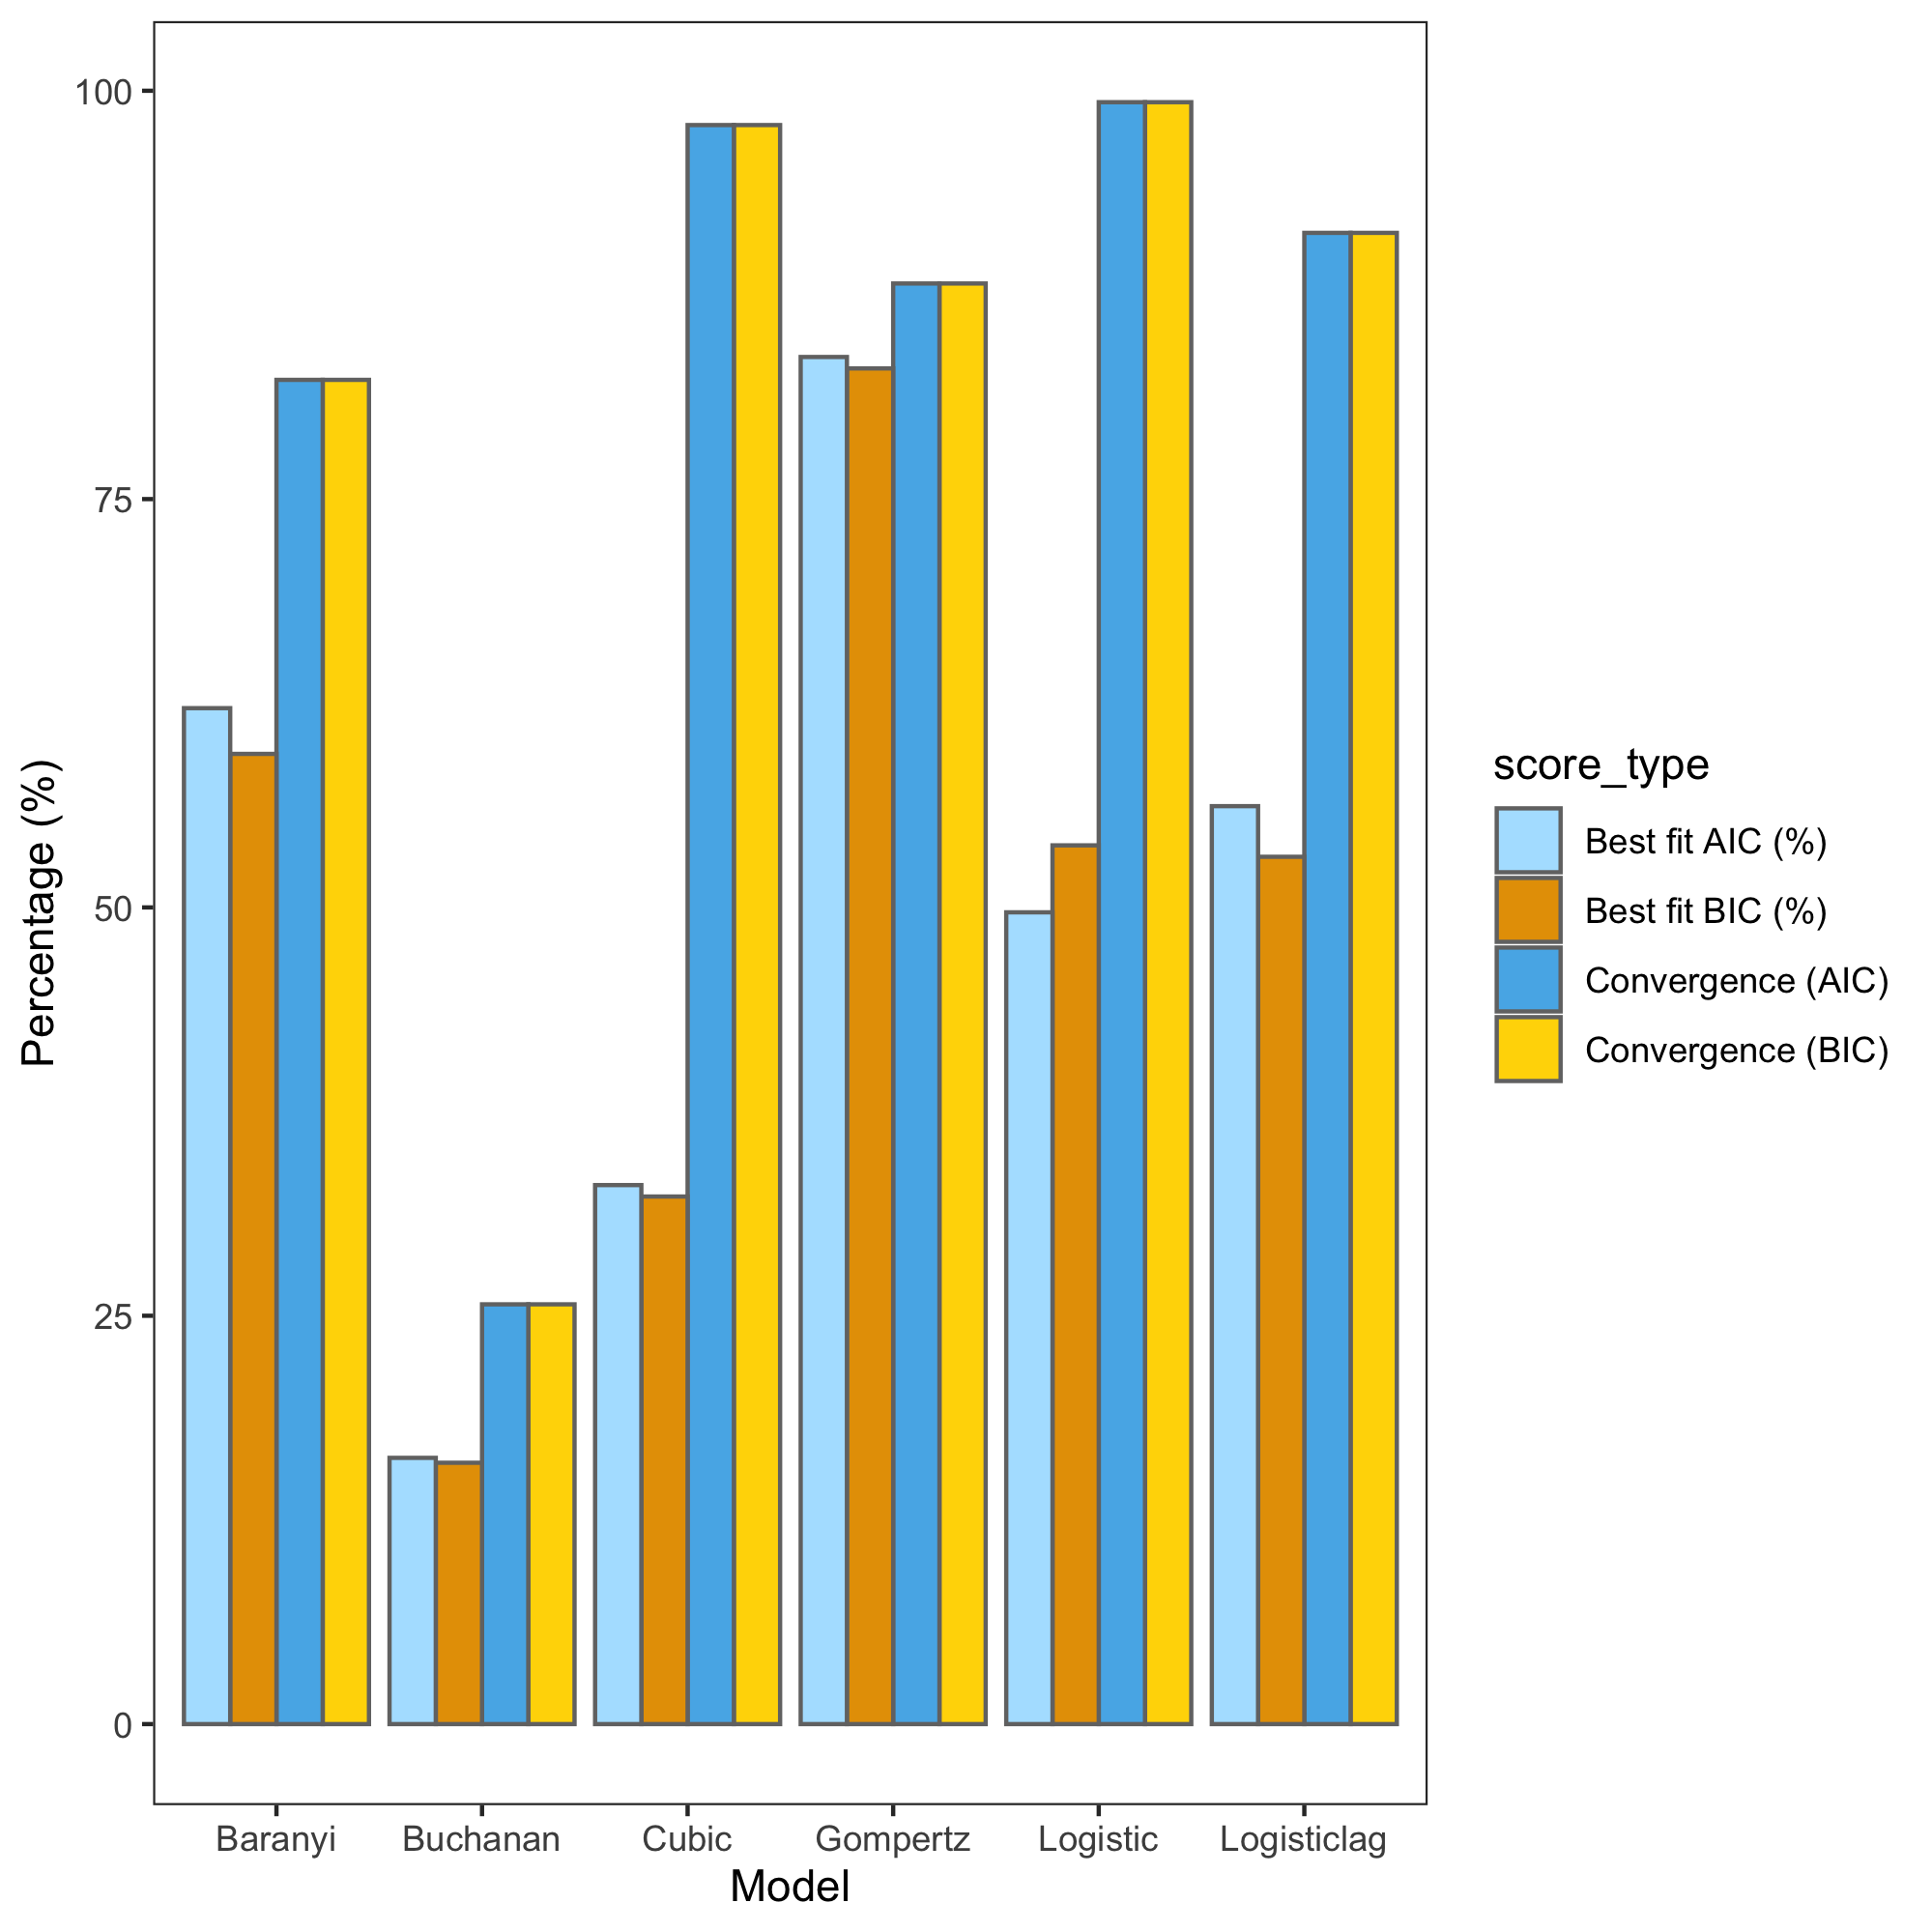
\includegraphics[width=\linewidth]{../results/stats.png}
                     \caption{Overall convergence and fitting score of candidate models}
                \end{center}
        \end{figure}
\begin{figure}[!ht]
            \centering
                \begin{center}
                    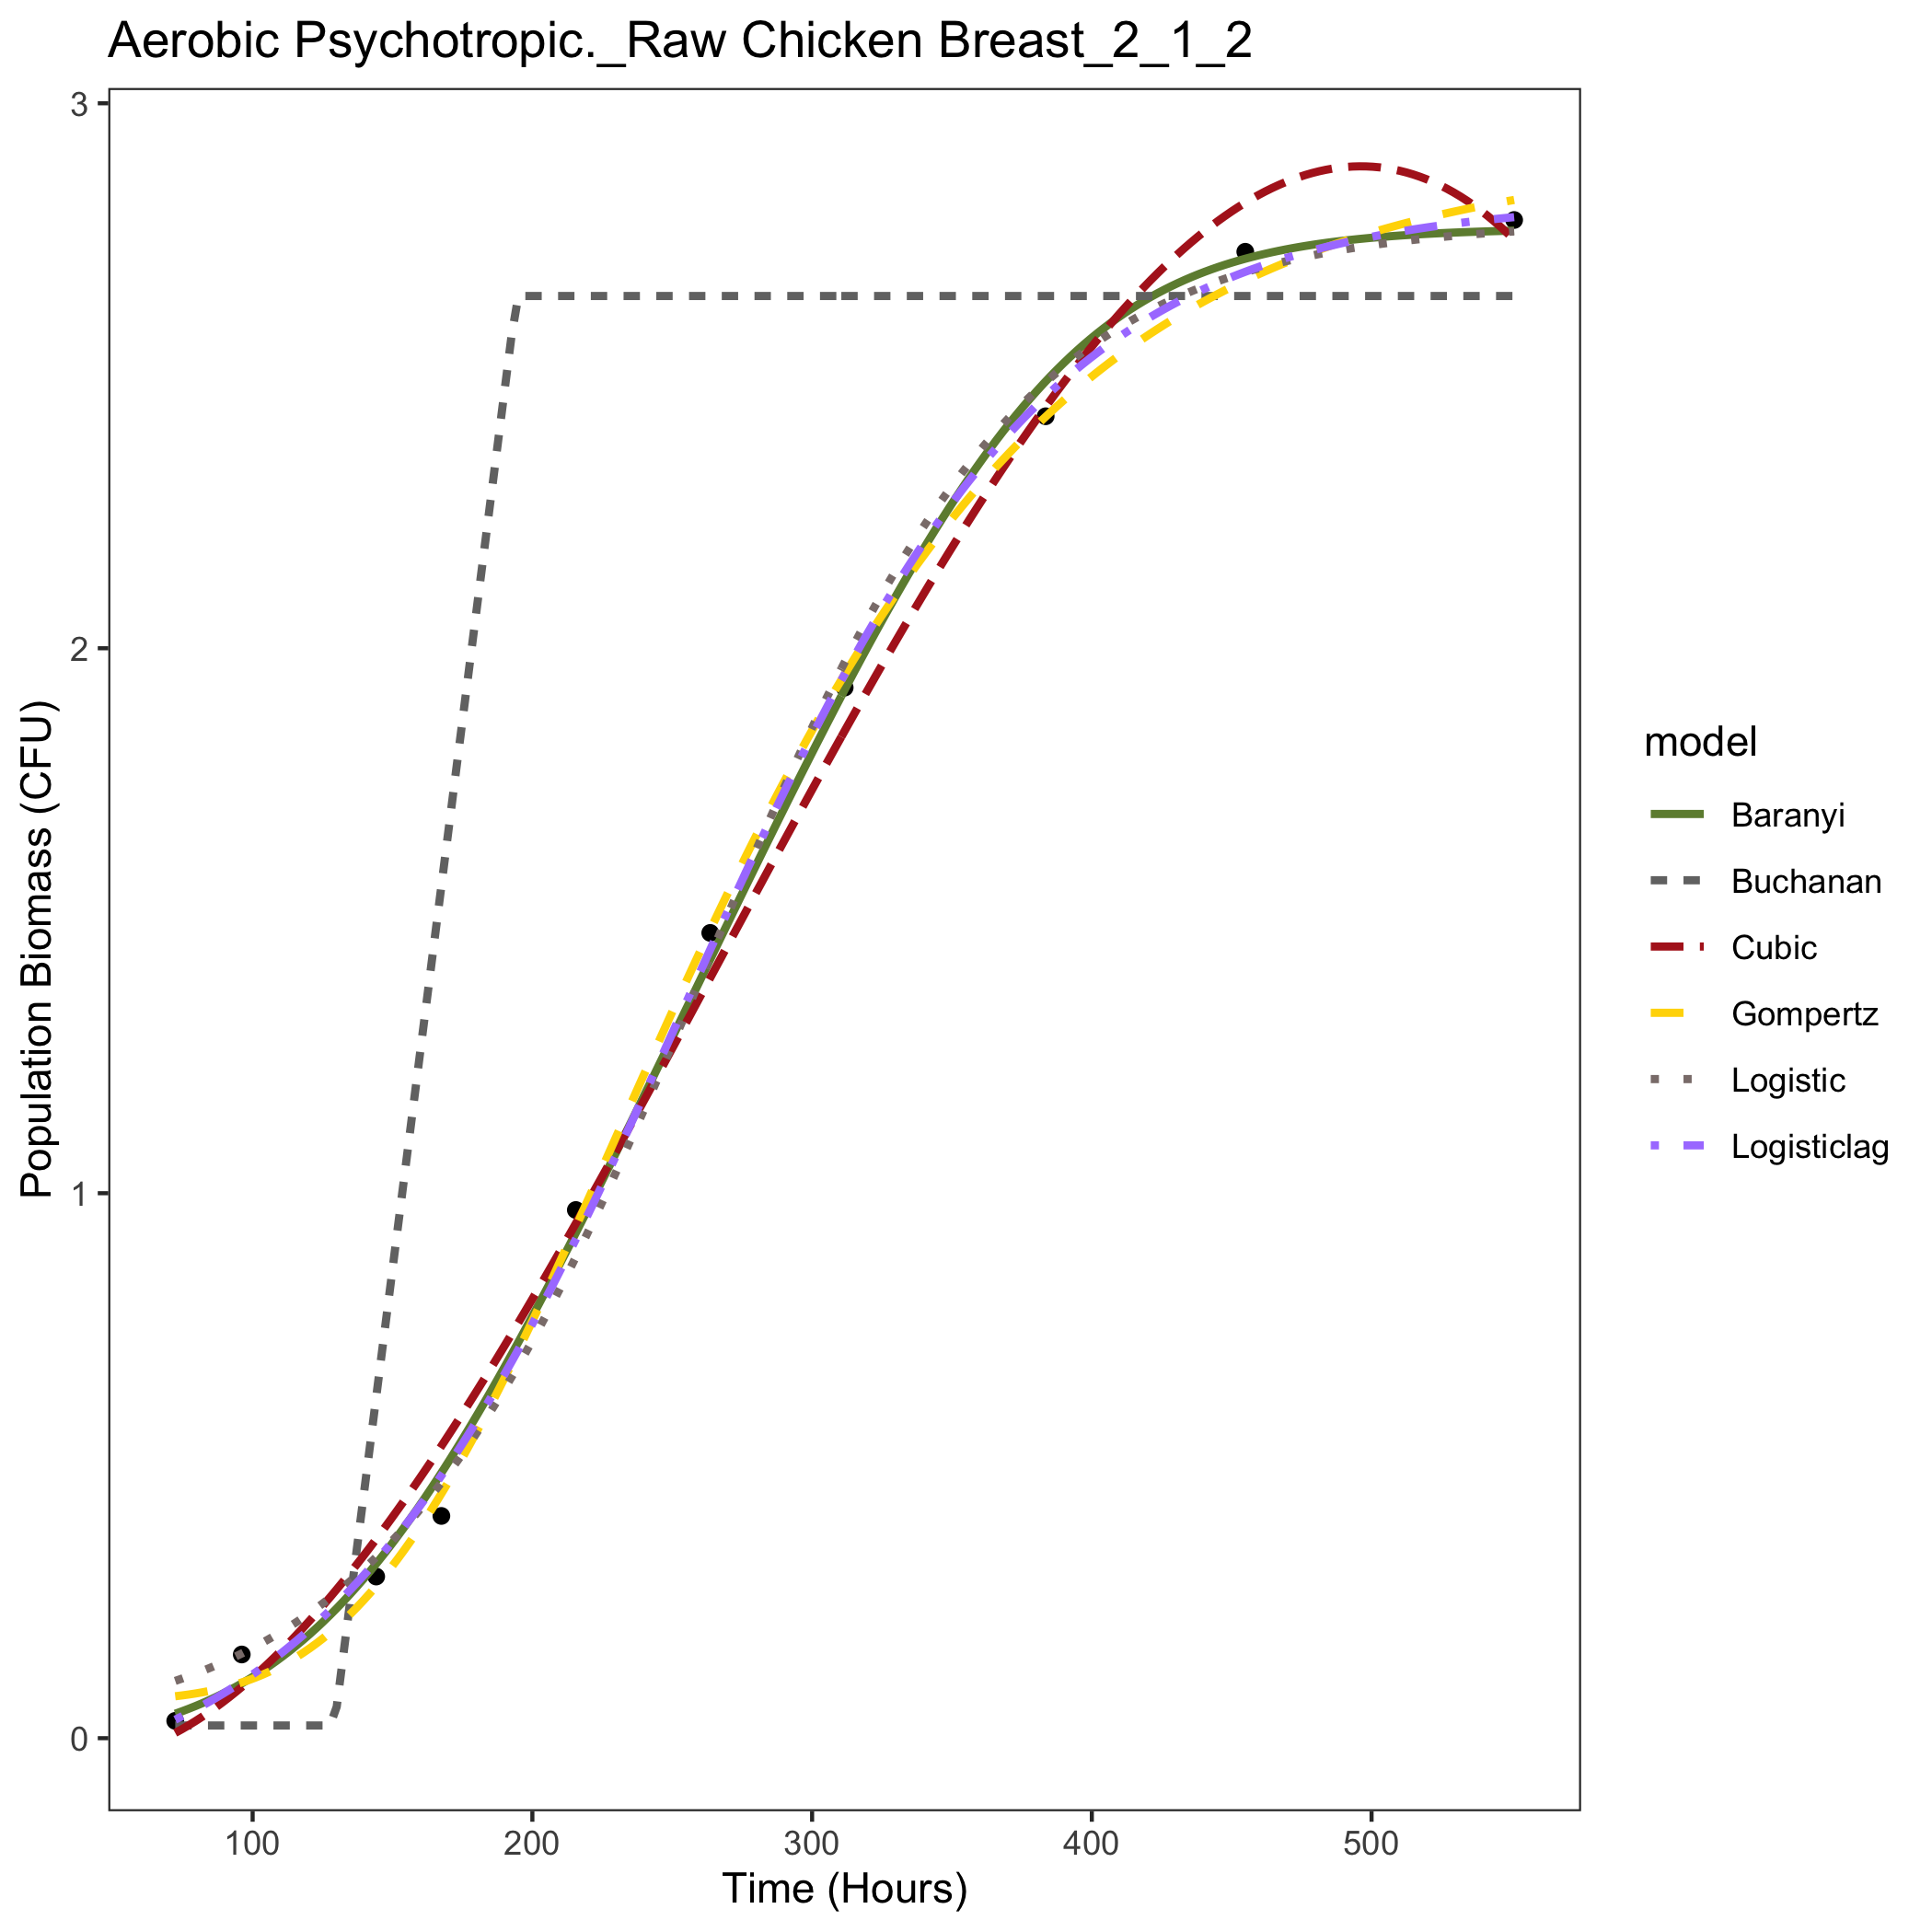
\includegraphics[width=\linewidth]{../results/example.png}
                     \caption{Growth curves of aerobic psychrotrophic bacteria in raw chicken breast at 2 \textdegree C fitted with 6 candidate models}
                \end{center}
        \end{figure}
\end{center}
\section{Discussion}
In this work, 5 models were compared statistically. The results showed that for the data used, the Gompertz model can be regarded as the most sufficient models among the candidates to best describe about 83\% of the subsets (Table 2). The AIC and BIC fitting scores gave a similar results overall. The BIC fitting scores of the two logistic models were close to each other while the AIC fitting score of logistic model with four parameters was higher than the one of logistic model with three parameters. This is reasonable as the penalty term for the number of parameters in the model is introduced in BIC. According to both AIC and BIC fitting, the three-parameter logistic model and the four-parameter logistic model performed almost the same.\\
Among all candidate models, the Buchanan model fitted the least number of subsets and received lowest fitting scores. The Buchanan model has been developed to emphasise the lag phase to help reconcile the known bacteria behaviour. However, the microbial data analysed in this work comes from various experiments which consist of different species grown in different conditions. The growth curves of the bacteria in this case does not always show a sigmoidal shape, which could gave difficulties fitting with the Buchanan model. The fact that the definition of lag is independent from the shape of the growth curve allows model with $t_{lag}$ parameter to model growth without a lag period, which could be the reason of the better performance of the Gompertz and the Baranyi model. \\
According to the analysis of the dataset in this study, the Gompertz model fitted the best. However, there could be imprecision when regard the Gompertz model as the best model. e.g., factors that have small effects for the majority of the cases but are significant in rare cases could be omitted \citep{levins1966strategy}. The comparison of different models for fitting growth curves across species is therefore important for gaining insights into the sufficient interpretation of biological phenomenon and providing accurate parameter estimates. Further needs in model building and model selection strategies should take into considerations of both the generality and precision, which is a contradictory demand and is essential for the understanding of population biology.

\end{linenumbers}

\bibliography{reference}
  
\end{document}